\documentclass[11pt]{article}
\usepackage{geometry}                % See geometry.pdf to learn the layout options. There are lots.
\geometry{letterpaper}                   % ... or a4paper or a5paper or ... 
%\geometry{landscape}                % Activate for for rotated page geometry
%\usepackage[parfill]{parskip}    % Activate to begin paragraphs with an empty line rather than an indent
\usepackage{graphicx}
\usepackage{amssymb}
\usepackage{epstopdf}
\usepackage{algorithm,algorithmic}
\DeclareGraphicsRule{.tif}{png}{.png}{`convert #1 `dirname #1`/`basename #1 .tif`.png}

\title{Notes on Table Driven - Bottom Up Parsers aka Simple LR Parsers}
\author{Daniel Beatty}
%\date{}                                           % Activate to display a given date or no date

\begin{document}
\maketitle
%\section{}
%\subsection{}


Parsing Concepts:
\begin{enumerate}
\item Syntax Directed Definitions
\item Translation Schemes
\end{enumerate}
Things these concepts have in common:
\begin{enumerate}
\item Both parse an input token stream
\item Build a parse tree
\item Traverse tree required to execute semantic actions
\end{enumerate}

Syntax directed definitions also have dependency graphs and syntax tree construction (page 284, 287).    Translation routines that are involved during parsing have two restrictions:
\begin{enumerate}
\item Grammar suitable for parsing may not be reflect the natural hierarchical structure of the langauage constructs.
\item Parsing method constrains the order in which nodes are evaluated.  
\end{enumerate}

\subsection {Action and Goto Tables} 
Thee is a generic algorithm that takes as input a matching action and goto table plus an input stream.  Its output is a parsed stream and state of acceptance.     (Cooke Lecture \#12 time 5:45)

Table based parsing has a stack, input stream.  These two determine the present state.  The algorithm consumes information from the input stream, pushes and pops information to the stack, and uses the states to determine whether a state and input are pushed on to the stack or whether to pop information off of the stack.    The shifts push states on to the stack, consumes the next token, and pushes that token on to the stack.   The shift information encoded in the table has the next state.     A reduce has both the production and sub-production indicated in the entry.   The size of the production determines how much to pop.  Also, if any semantic actions occur at the end of the production, then those get called as well.  Note that table based parsing forbids ``embedded semantic actions''.   

\begin{figure}[htbp] %  figure placement: here, top, bottom, or page
   \centering
   \includegraphics[width=4in]{actionTable.pdf} 
   \caption{Action Table for example grammar}
   \label{fig:actiontable}
\end{figure}

\begin{figure}[htbp] %  figure placement: here, top, bottom, or page
   \centering
   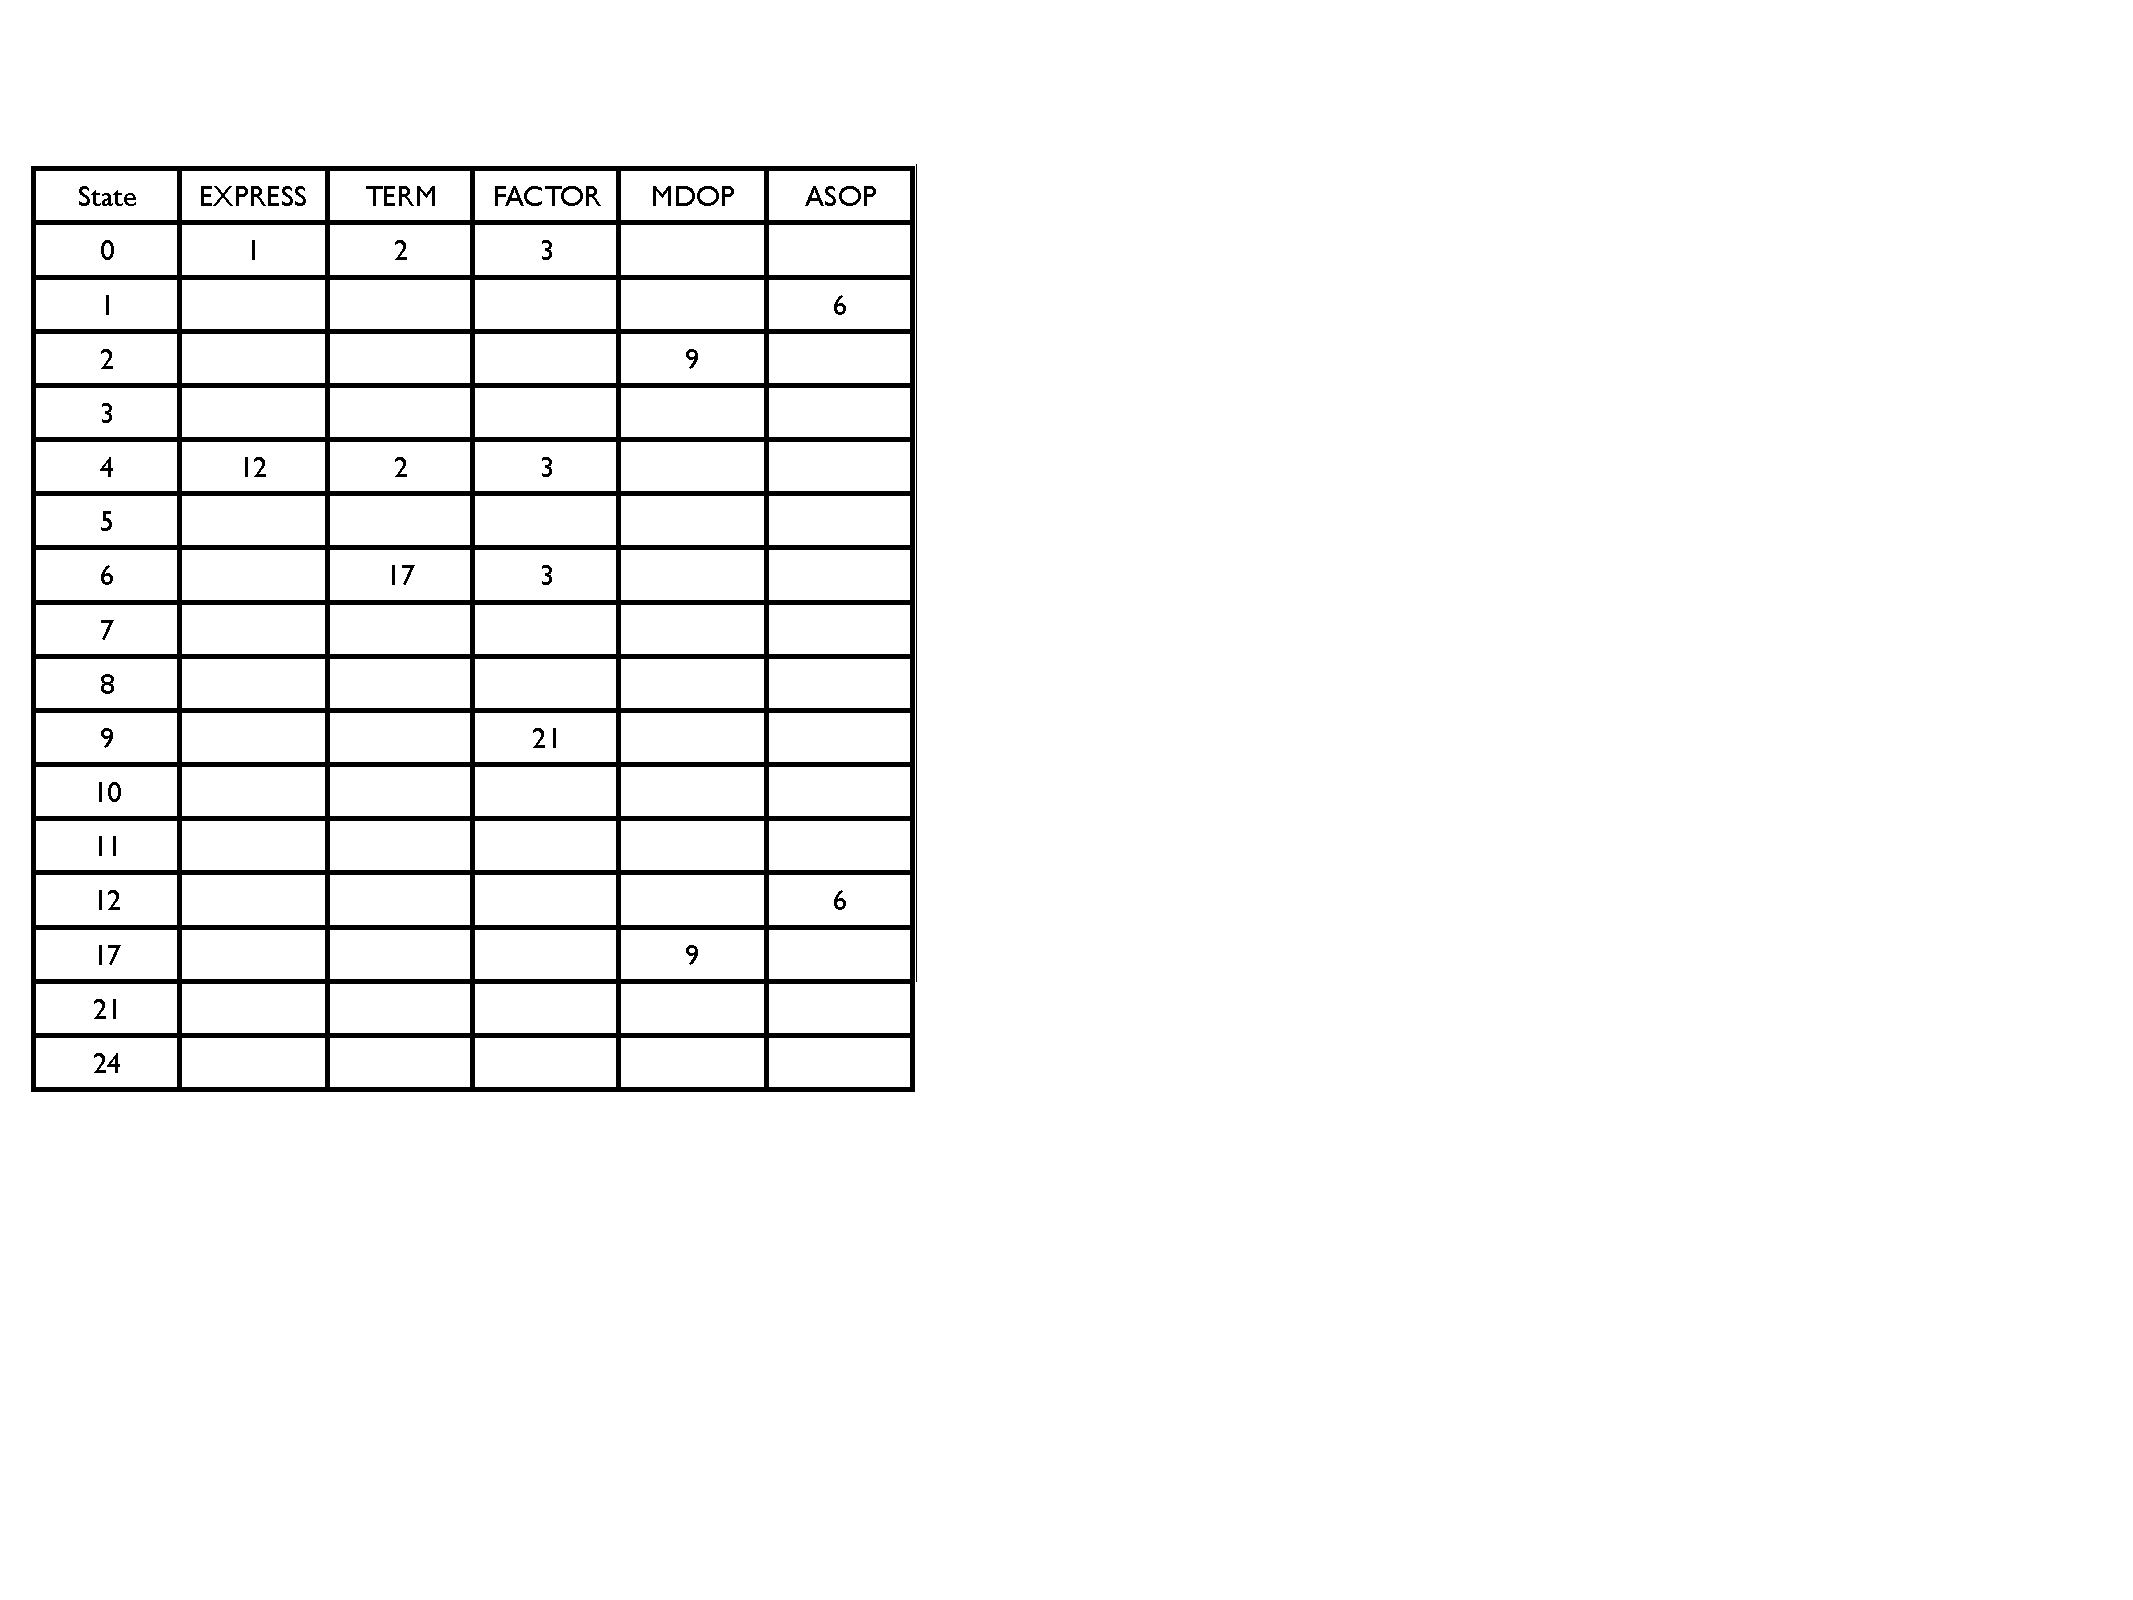
\includegraphics[width=4in]{gotoTable.pdf} 
   \caption{Goto table for example grammar}
   \label{fig:gotoTable}
\end{figure}



\begin{figure}[htbp] %  figure placement: here, top, bottom, or page
   \centering
   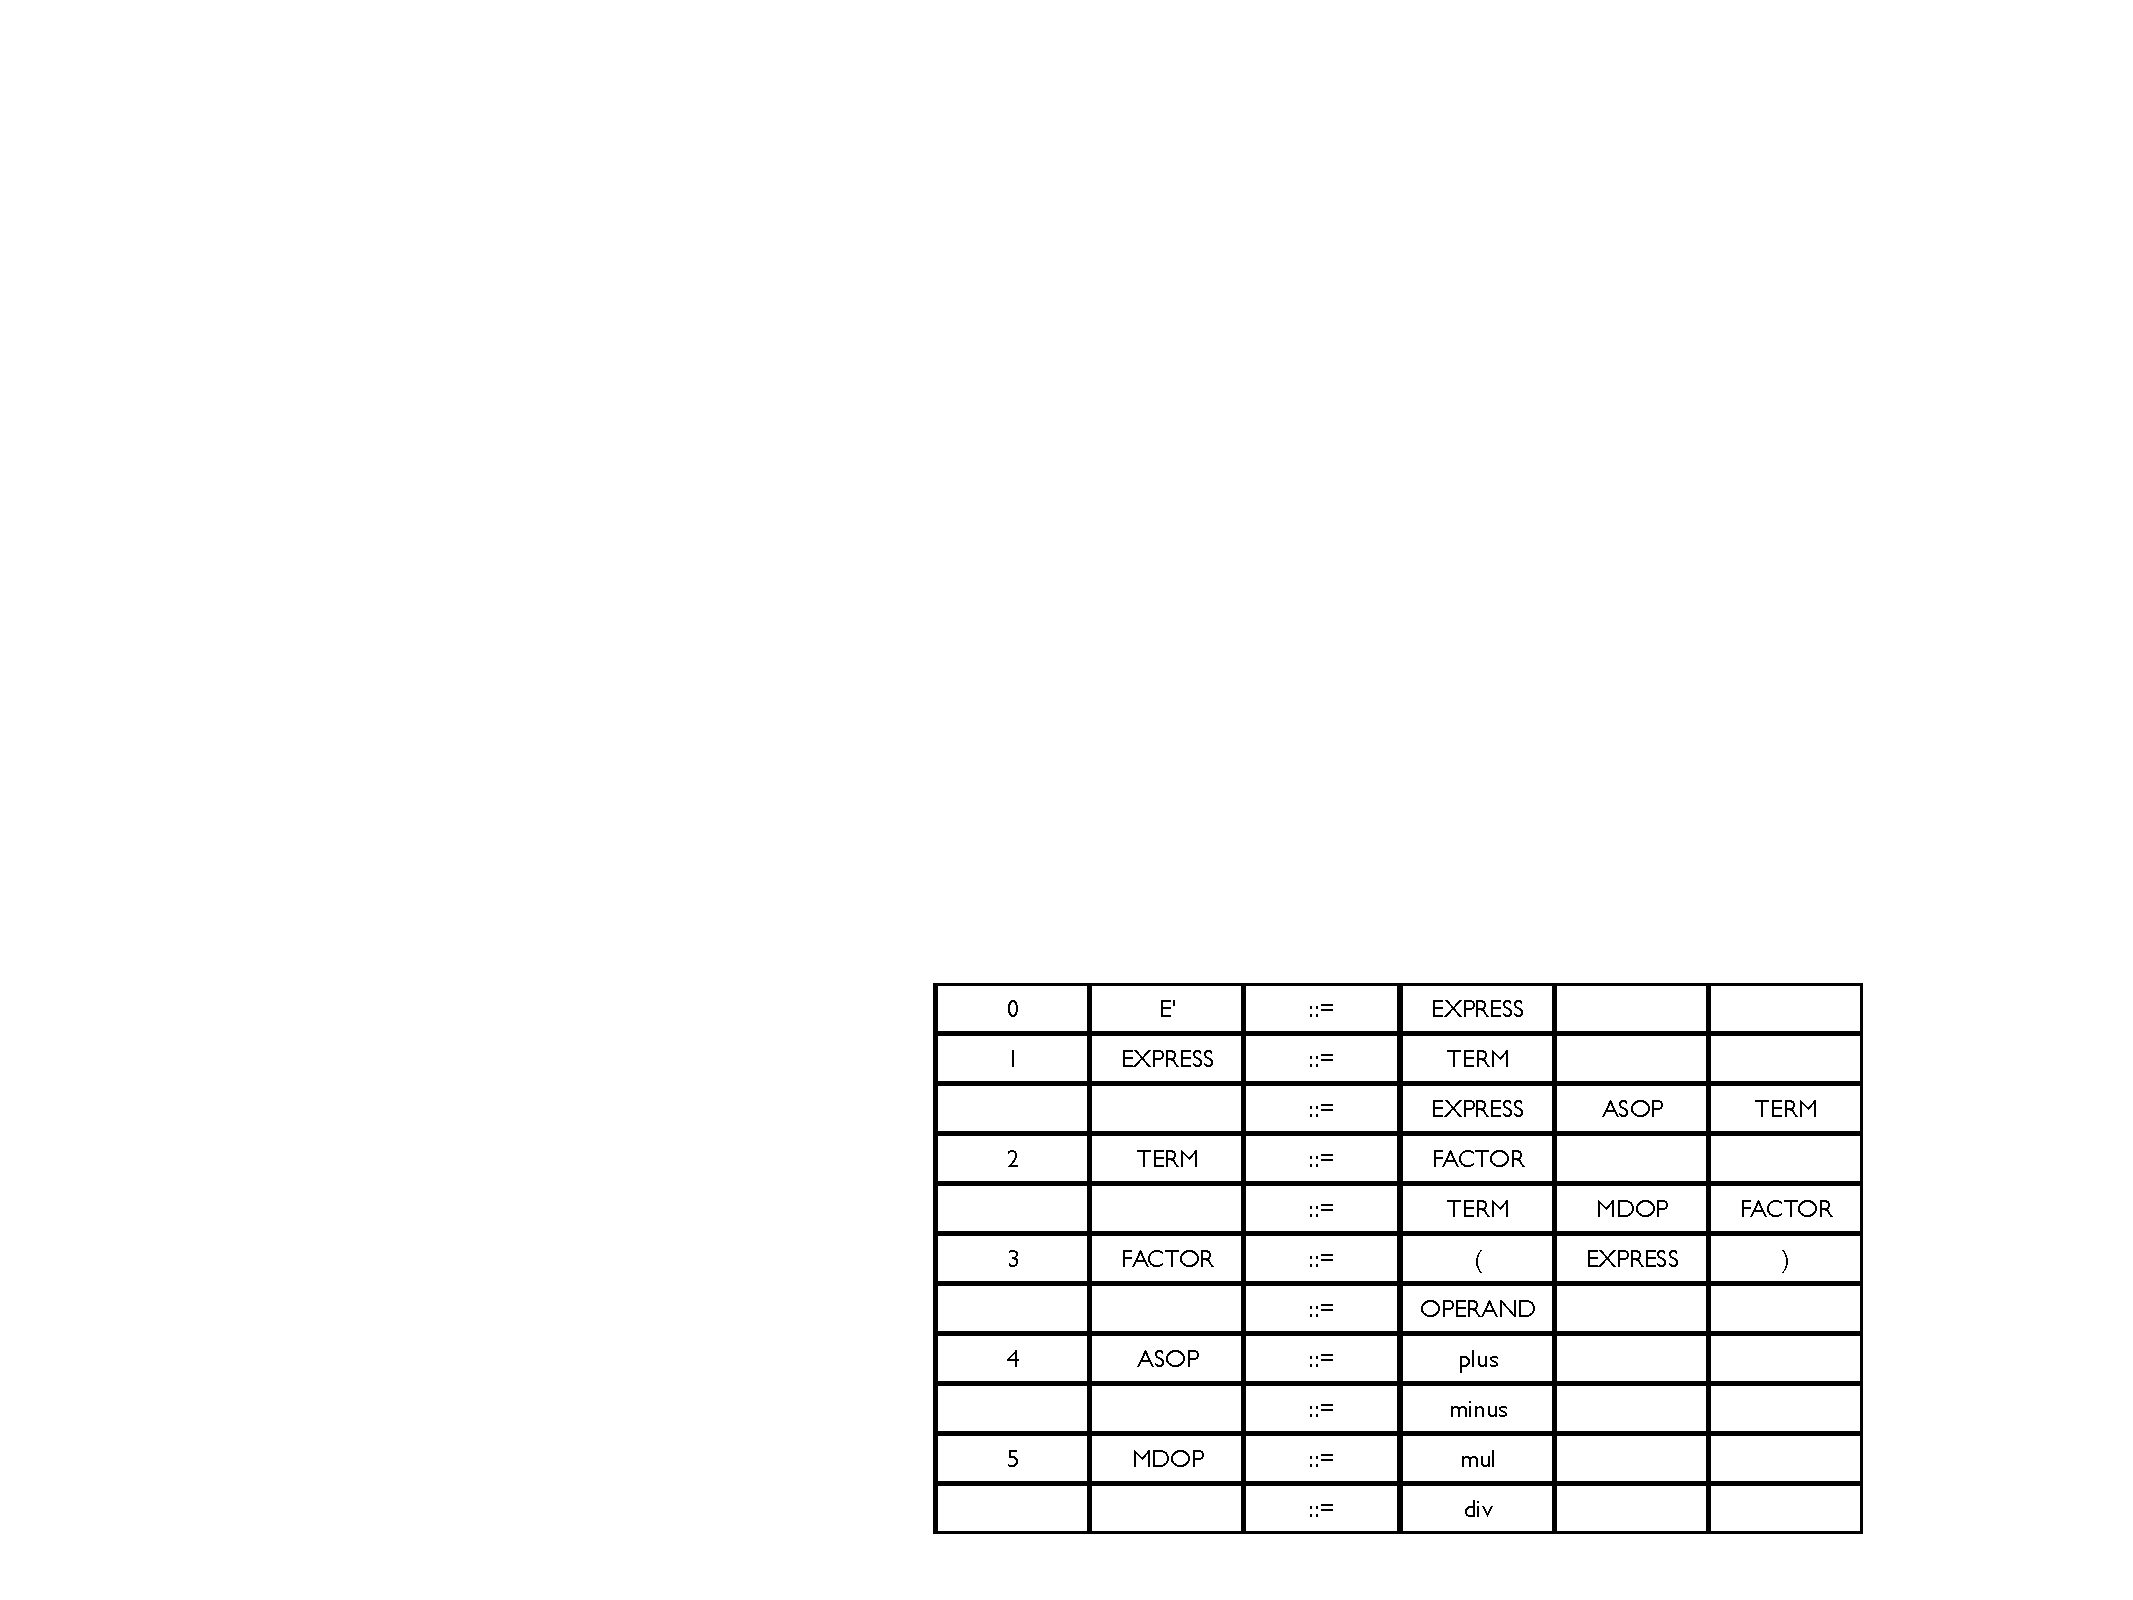
\includegraphics[width=4in]{reductionTable.pdf} 
   \caption{Reduction Table for an Example Grammar}
   \label{fig:reductionTable}
\end{figure}

A good question is does table based semantics allow for epsilon productions which could be embedded which would generate ``embedded semantic actions?''  Answers is yes, but why do it.  The only conceivable benefit has to do with embedded semantic actions.  An $\epsilon$ production may be a good choice in these categories since they force selections to handle them.  A compromise would be short ``cheese'' embedded productions which are not necessary for the syntax, but payoff in the semantic action section.  




\begin {algorithm}
\caption{ Table Driven Parse }
\label{alg:NU}
\begin{algorithmic}
\STATE ACCEPT:=FALSE;
\STATE ERROR := FALSE;
\STATE push ($s_0$) 
\REPEAT
\STATE Examine next input symbol = $a_i$  and state $s_m$ = TOP(Stack);
\IF {ACTION[s m , a i ] = a.  shift s }	
\STATE consume a i
\STATE push(a i)
\STATE push(s )
\ELSE \IF {reduce $B \to \beta$ }
\STATE  pop $2r$ items from stack where $r = | \beta | $ 
\STATE $s = \textrm{GOTO}[s m � r , B]$ where s, m � r = TOP(stack after the 2r items are popped)
\STATE push(B)
\STATE push(s )
\ELSE \IF  {accept }	\STATE	ACCEPT:=TRUE
\ELSE \IF {error }	\STATE	ERROR:=TRUE
\ENDIF
\ENDIF
\ENDIF 
\ENDIF
\UNTIL {ACCEPT or ERROR}

\end{algorithmic}
\end{algorithm} source (Cooke's lecture, and Knuth's Dissertation)

\newpage
Semantic actions can only occur in reductions, in particular at the end of the reductions.  
The heavy lifting by the Table Driven Parse is done by the shifts and reduce.    The three actions for a shift are:
\begin{enumerate}
\item consume $a_i$: \\
This function calls the lexical analyzer's lex operation.  As a result, the value of $a_i$ is made available to the algorithm.  
\item  push($a_i$) \\
The $a_i$ is pushed on to the parsing stack.  
\item push($s_i$) \\
Both the current state and next state are available as result of the iteration of the algorithm.   These two states were made available by the top of the stack which has a state at the end of each iteration, and the reference into the action table.    The reference into the token are from the state $s_m$ from the top of the stack, and the consumed token $a_i$.    %The four operations of this algorithm are encoded actions present in the action table.  Those action also contain specifics of the action such as reduce production 3 sub production 2, symbolized  by R3.2.     
In the case of the shift encoding, the next state is also include which is denoted by $s_i$.  This $s_i$ is pushed and will be referenced in the next iteration.  
\end{enumerate}

In the case of reduce, the elements included with the production are $B$ which is the production, and $beta$ the specific sub-production of $B$.    The consequences of this reduction action are as follows:
\begin{enumerate}
\item  pop $2r$ items from stack where $r = | \beta | $  \\
Every sub-production has a length (number of terminals and non-terminals).  The value for this is 
$r = | \beta |$.  The parsing stack is simply popped $2r$ times.  The values of this popping may be stored in array and sent into semantic analyzer as an argument for the semantic action associated with the production.  
\item  $s = \textrm{GOTO}[s_{ m � r} , B]$  \\where $s_{ m � r} = TOP$ (stack after the 2r items are popped).  Note that the first operation popped off the elements associated with a sub-production.   The goto table has reference information for the current stack top state $s_{m-r}$ and where the input stream could be next.  

\item  push(B) \\
The production itself is pushed and happens to define particular action that may be used later in some semantic action.
\item  push(s ) \\  The goto state is pushed and is the next top state for use in the next iteration.  
\end{enumerate}

One use analysis of Dr. Knuth's algorithm is the complexity of this algorithm.   The complexity is based off of the number of productions and the length of the input stream (token wise).   Error recovery may also be a useful analysis of this algorithm.  

\textbf{Example:} Try the example tables with the following sentence in the calculator grammar:
\begin{center}
a + b
\end{center}
As a result the following table is generated indicating the steps taken during the execution of Dr. Knuth's algorithm.
\begin{table}[htdp]
\caption{Example execution of Dr. Knuth's algorithm for \textrm{a + b} in the calculator grammar. }
\begin{center}
\begin{tabular}{|l|l|l|l|l|}
Step 	& Stack (left to right) & Input Stream & Action table value \\
1		& $S_0$		& a + b \$ & $S_5$	\\
2	&	$S_0$ a $S_5$	&	+ b \$	&   R3.2 \\
% Factor -> Operand  
% Length 1  , r = 2
3	&	$S_0$, Factor , $S_3$	&	+ b \$ & R2.1 \\
% Another reduction 
% Term -> Factor (aka B3) r = 2
4	&	$S_0$ , Term , $S_2$	&	+ b \$ & R1.1	\\
% reduction for expression 
% expression -> term r = 2 
5 	& $S_0$ , Express, $S_1$	& + b \$	& S7 	\\
% Shift 7
6	& $S_0$ , Express, $S_1$, +, $S_7$ &  b \$ &  R4.1 \\
7	& $S_0$ , Express, $S_1$, ASOP, $S_6$ & b \$ &  S5 \\
8	& $S_0$ , Express, $S_1$, ASOP, $S_6$ b $S_5$ &  \$ &  R3.2 \\
9	& $S_0$ , Express, $S_1$, ASOP, $S_6$, Factor, $S_3$ &  \$ &  R2.1 \\
10	& $S_0$ , Express, $S_1$, ASOP, $S_6$, Term $S_{17}$ &  \$ &  R1.2 \\
11	& $S_0$ , Express $S_1$ &  \$ &  Accept \\
\end{tabular}
\end{center}
\label{default}
\end{table}%




\newpage
Again, the calculator grammar under table parsing can not use embedded semantic actions without embedding simple productions.   In this case, there is such a thing.  The ASOP and MDOP productions are simple productions for plus, minus, multiply and divide symbols.   A push operation on the semantic action stack can be used with these productions.    The factor is a little more complex.  In its operand production, it is also a push.  However, most of it is simply reclaiming items from the semantic action stack.   It is the reclaiming that allows such semantic actions to properly process what is parsed.  In the case of terms and expressions, they reclaim both the operation and operands from the semantic action stack.  Thus Knuth's algorithm is augmented to include semantic actions:


\begin {algorithm}
\caption{ Table Driven Parse with Semantic Action Calls }
\label{alg:NU}
\begin{algorithmic}
\STATE ACCEPT:=FALSE;
\STATE ERROR := FALSE;
\STATE push ($s_0$) 
\REPEAT
\STATE Examine next input symbol = $a_i$  and state $s_m$ = TOP(Stack);
\IF {ACTION[s m , a i ] = a.  shift s }	
\STATE consume a i
\STATE push(a i)
\STATE push(s )
\ELSE \IF {reduce $B \to \beta$ }
\STATE Semantic Action for $B \to \beta$.
\STATE  pop $2r$ items from stack where $r = | \beta | $ 
\STATE $s = \textrm{GOTO}[s m � r , B]$ where s, m � r = TOP(stack after the 2r items are popped)
\STATE push(B)
\STATE push(s )
\ELSE \IF  {accept }	\STATE	ACCEPT:=TRUE
\ELSE \IF {error }	\STATE	ERROR:=TRUE
\ENDIF
\ENDIF
\ENDIF 
\ENDIF
\UNTIL {ACCEPT or ERROR}

\end{algorithmic}
\end{algorithm} source (Cooke's lecture, and Knuth's Dissertation)


\begin{table}[htdp]
\caption{Productions and Semantic Rules for the example calculator grammar}
\begin{center}
\begin{tabular}{|l|l|l|l|}
Production Number & Production & Follow Set & Semantic Rules \\
0	&	$E' \to E$ & & \\
1. 	&	$E \to T$ & +, - ) \$   &\\
 	& 	$E \to EAT $ &  & [imCode op ]\\
	\hline
2. 	&	$T \to F$	& + , - , *, div , ) \$ & \\
	&	$T \to TMF$ & & [imCode op ] \\
	\hline
3.	&	$F \to ( E ) $ 	& + , - , *, div , ) \$  &\\
	&	$F \to o_p $ & & [imCode p ] \\
	\hline
4.	&	$A \to + $	& $o_p$ , (  & [imCode p ] \\
	&	$A \to -$ 	&  & [imCode p ] \\
	\hline
5	&	$M \to *$ 	& $o_p$ , (  & [imCode p ] 	\\
	&	$M \to \textrm{div} $ &  & [imCode p ] \\
\end{tabular}
\end{center}
\label{default}
\end{table}%
\textbf{Another example:}  ( a + b ) * c .  Also genquads for the following actions:


\begin{table}[htdp]
\caption{Another example for \textrm{( a + b ) * c }}
\begin{center}
\begin{tabular}{|l|l|l|l|l|}
Step &	Stack &	Input	& State \\
1	& $S_0$	&	(a + b ) * c \$ &	S4 \\
2	& $S_0$ ( $S_4$	&	a + b ) * c \$ &	S5 \\
3	& $S_0$ ( $S_4$ a $S_5$	&	 + b ) * c \$ &	R3.2 \\
4	& $S_0$ ( $S_4$ F $S_3$ &	 + b ) * c \$ &	R2.1 \\
5	& $S_0$ ( $S_4$ T $S_2$   &	 + b ) * c \$ &	R1.1 \\
6	& $S_0$ ( $S_4$ E $S_{12}$  &	 + b ) * c \$ &	S7 \\
7	& $S_0$ ( $S_4$ E $S_{12}$ + $S_7$  &	  b ) * c \$ &	R4.1 \\
8	& $S_0$ ( $S_4$ E $S_{12}$ A $S_6$  &	  b ) * c \$ &	S5 \\
9	& $S_0$ ( $S_4$ E $S_{12}$ A $S_6$  b $S_5$ &	   ) * c \$ & R3.2	 \\
10	& $S_0$ ( $S_4$ E $S_{12}$ A $S_6$  F $S_3$ &	   ) * c \$ & R2.1	 \\
11	& $S_0$ ( $S_4$ E $S_{12}$ A $S_6$  T $S_{17}$ &	   ) * c \$ & R1.2	 \\
12	& $S_0$ ( $S_4$ E $S_12$ &	   ) * c \$ & S24	 \\
13	& $S_0$ ( $S_4$ E $S_12$ ) $S_{24}$ &	    * c \$ & 	 R3.1 \\
14	& $S_0$ F $S_3$ &	    * c \$ & 	 R2.1 \\
15	& $S_0$ T $S_2$ &	    * c \$ & 	 S10 \\
16	& $S_0$ T $S_2$ * $S_{10}$ &	    c \$ & 	 R5.1 \\
17	& $S_0$ T $S_2$ M $S_9$ &	    c \$ & 	 S5 \\
18	& $S_0$ T $S_2$ M $S_9$ c $S_5$ &	     \$ & 	R3.2  \\
19	& $S_0$ T $S_2$ M $S_9$ F $S_{21}$ &	     \$ & 	R2.2  \\
19	& $S_0$ T  $S_2$ &	     \$ & 	R1.1  \\
20	& $S_0$ E $S_1$ &	     \$ & 	Accept  
\end{tabular}
\end{center}
\label{default}
\end{table}%

Examples from Ullman, page 190-192 and 216-220

\newpage
\subsection{Constructing the Simple Left to Right Shift Reduce (SLR) Parsing Table} 
The key for Simple LR parsing to work is to use an algorithm that recognizes viable prefixes  of the grammar.  This is done by using tables (action and goto) which is derived from a deterministic  finite automation.  Ullman places in a disclaimer with this algorithm in that ``will not produce uniquely defined parsing action tables for all grammars''.    LL1 is not a problem.  Context Free Grammars are not a problem.    Follow sets are required for this grammar.   First sets are not.  However, first and follow sets will yield selection sets.  However, the LL1 condition is not required on these first and follow sets.  

\begin{itemize}
\item Given a grammar $G$, apply an augment $G'$ that produces $G$.  
\begin{itemize}
\item ``if $G$ is a grammar with start symbol $S$, then $G'$ , then $G'$, the \textsl{augmented grammar} for $G$, is $G$ with a new start symbol $S'$ and production $S' \to S$. ''
\item ``The purpose of this new starting productions is to indicate to the parser when it should stop parsing and announce acceptance of the input.'' 
\end{itemize}

\item The ``LR parser can determine from the state on top of the stack everything that it needs to know about what is in the stack.''  Furthermore a ``grammar that can be parsed by an LR parser examining up to $k$ input symbols on each move is called an LR(k) grammar.'''  

\item ``An LR(0)  item (item for short) of a grammar $G$ is a production of $G$ with a dot at some position of the right side.'' 
\item The central idea for the SLR parser is ``first construct from the grammar a deterministic finite automaton to recognize viable prefixes.''   
\item canonical LR(0) collections provides the basis for constructing SLR parsers.  
\item Closure categories:
\begin{itemize}
\item \textsl{Kernel item } include the initial item, and all items whose dots are not at the left end. 
\item \textsl{Nonkernel items} which have their dots at the left ends.  
\end{itemize}

\end{itemize}



\begin {algorithm}
\caption{ Function collection(G:grammar): collection of sets of items }
\label{alg:collection}
\begin{algorithmic}
\STATE Collection:= \{Closure($\{A� \to .A\}$) \};
\REPEAT
\STATE For each set of items I in Collection and each symbol X 
\IF { GOTO (I,X) $\neq$ null  is not in Collection} 
	\STATE Add GOTO(I,X) to Collection; \ENDIF
	
\UNTIL {no more I�s are added to Collection}
\RETURN Collection
\end{algorithmic}
\end{algorithm}

The collection algorithm uses the augmented production to start the Collection process.   The closure function will move the period around.  Intuitively this period can be thought of as a special delimiter.  It allows for all of the LR(0) items to be found.  

\begin {algorithm}
\caption{ Function Closure(I:set of Items): set of items; }
%\REMARK $\alpha$ and $\beta$ may be any collection of terminals, and non-terminals.  They may also be empty.  
\label{alg:closure}
\begin{algorithmic}
\REPEAT
\STATE For each item $B \to \alpha . C \beta \in I$ and each production $C\to \gamma \in G$
\IF { $C \to . \gamma \ni I $ }
	\STATE Add $C \to . \gamma $ to $I$;
\ENDIF
	
\UNTIL {no more items can be added to $I$}
\RETURN Closure := I; 
\end{algorithmic}
\end{algorithm}



\begin {algorithm}
\caption{ Function Goto(I:set of Items, X: symbol in the grammar ): set of items; }
\label{alg:closure}
\begin{algorithmic}
\STATE S = \{ \} ;
\FORALL {$B \to \alpha . X \beta \in I$ }
\STATE S := $S \cup $ Closure ( $\{ B \to \alpha X. \beta \} $ )
\ENDFOR
\RETURN goto := S; 
\end{algorithmic}
\end{algorithm}


\begin {algorithm}
\caption{ Function Action Tables }
\label{alg:actionTables}
\begin{algorithmic}
\IF {$[B \to \alpha .b \beta ] \in I_i$ and $\textrm{GOTO}(I_i , b ) = i_j$ } 
\STATE $\textrm{ACTION}[i,b] := s_j$
\ENDIF
\IF {$[ B \to \alpha . ] \in l_i ]$ } 
\STATE $\textrm{ACTION}[i,b] := r_n$
\ENDIF
\end{algorithmic}
\end{algorithm}

\newpage
\textbf{Creating Action Table}
\begin{enumerate}
\item if  $[B \to \alpha .b \beta ] \in I_i$ and $\textrm{GOTO}(I_i , b ) = i_j$ , then $\textrm{ACTION}[i,b] := s_j$
\item if $[ B \to \alpha . ] \in l_i ]$ then $\textrm{ACTION}[i,b] := r_n$ for all $b \in \textrm{FOLLOW}(B) $ and where $n$ is the number of $B \to \alpha$
\item if $[ A' \to A. ] \in l_i $  then $\textrm{ACTION}[i,\$] := \textrm{ACCEPT}$.
\end{enumerate}

Indicies into grammar comment at 44:24



The shift actions are fairly straight forward.  The follow sets can be a bit confusing.  

The first example of this occurs in $I_2$ where $E \to T.$ is found.  This corresponds to production 1.1.  Consequently, that production number is also the $n$ of $r_n$.  

\begin{table}[htdp]
\caption{Example: The Calculator Grammar and its goto table}
\begin{center}
\begin{tabular}{|l|l|l|}
\textbf{Item} & \textbf{Production}	& \textbf{Actions} \\
$I_0$ & $E' \to .E$ & Establish Collection with Closure ($E\to .E$) \\
	& $E \to .T $	&	\\
	& $E \to .EAT $		&	\\
	& $T \to .F $	&	\\
	& $T \to .TMF $	&	\\
	& $F \to .( E ) $ 	&	\\
	& $F \to .o_p$ 	&	\\
\hline
$I_1$ &  $E' \to E.$ & Apply Goto ($I_0$, E) \\
	& $E' \to E. $	&\\
	& $E \to E.AT $		& Apply to $A$	\\
	& $A \to .+ $		&	\\
	& $A \to .- $		&	\\
\hline
$I_2$ &  $E \to T.$ & Apply Goto ($I_0$, T) \\
	&  $T \to T.MF$ &  Closure on $.M$\\
% Note the reduction qualities of this production
	&  $M \to .* $ & \\
	&  $M \to ./ $ &  \\
\hline 
$I_3$ &  $T \to F. $	& Apply Goto ($I_0$, F), no closure	\\	
\hline
$I_4$ &  $F \to ( .E ) $ & Apply Goto ($I_0$, ( ) 	\\
	& $E \to .T $	&	\\
	& $E \to .EAT $		&	\\
	& $T \to .F $	&	\\
	& $T \to .TMF $	&	\\
	& $F \to .( E ) $ 	&	\\
	& $F \to .o_p$ 	&	\\
\hline
$I_5$ &  $F \to o_p.$  & Apply Goto ($I_0$, $o_p$ ) 	\\
\hline
$I_6$ &  $E \to EA.T $  & Apply Goto ($I_1$, $A$ ) 	\\
	&  $T \to .F $  & closure	\\
	&  $T \to .TMF $  &	\\
	&  $F \to .(E) $  &	\\
	& $F \to .o_p$ 	&	\\
\hline
$I_7$ & $A \to +. $  & Apply Goto ($I_1$, $+$ ) 	\\
\hline
$I_8$ & $A \to -. $  & Apply Goto ($I_1$, $-$ ) 	\\
\hline
$I_9$ & $T \to TM.F $ & Apply Goto ($I_2$, M) \\
	& $ F \to .(E) $ & Closure on $.F$ \\
	& $F \to .o_p$ &	\\
\hline
$I_{10}$ &	$M \to *. $	&	Apply Goto ($I_2$, * ) \\
$I_{11}$ & $M \to /.$ &	Apply Goto ($I_2$, / ) \\
\hline

\end{tabular}
\end{center}
\label{default}
\end{table}%

\begin{table}[htdp]
\caption{Example: The Calculator Grammar and its goto table continued}
\begin{center}
\begin{tabular}{|l|l|l|}
\textbf{Item} & \textbf{Production}	& \textbf{Actions} \\
\hline
$I_{12} $ &   $F \to ( E. ) $	& Apply Goto ($I_4$, .E ) \\
		& $E \to E.AT $ & Apply closure on $A$ \\
		& $A \to .+ $	&	\\
		& $A \to .- $	&	\\
		
\hline
$I_{13} $ &   $E \to T. $	& Apply Goto ($I_4$, T ) = $I_2$ \\
\hline
$I_{14} $ &   $T \to F. $	& Apply Goto ($I_4$, F ) = $I_3$ \\
\hline
$I_{15} $ &   $F \to (.E) $	& Apply Goto ($I_4$, ( ) = $I_4$ \\
\hline
$I_{16} $ &   $F \to o_p . $	& Apply Goto ($I_4$, ( ) = $I_5$ \\
\hline 
$I_{17}$ & $E \to EAT. $ 	& GOTO ( $I_6$, T) \\
	&  $T \to T.MF $  &	 Closure on $M$ \\
	& $M \to * $	& \\
	& $M \to / $	& \\
\hline 
$I_{18}$ & $T \to F. $  & GOTO ($I_6$, F) =  $I_3$ 	\\
\hline 
$I_{19}$ &  $F \to (.E) $  &	 GOTO ($I_6$, ( ) = $I_4$\\
\hline 
$I_{20}$ &  $F \to o_p.$   &	 GOTO ($I_6$, $o_p$ ) = $I_5$\\
\hline 
$I_{21}$ &	$T \to TMF.$ &	GOTO ($I_9$, F)  \\
\hline 
$I_{22} $&  $F = (. E )$  &Apply GOTO ($I_9$, ( ) =  $I_4$ \\
\hline 
$I_{23}$ & $F \to o_p .$ &Apply GOTO ($I_9$, $o_p$ ) =  $I_5$ \\
\hline 
$I_{24}$ &  $F \to ( E ) . $  &GOTO ($I_{12}$, ) ) \\
\hline 
$I_{25}$ &  $E \to EA.T. $  &GOTO ($I_{12}$, A ) = $I_6$ \\
\hline 
$I_{26}$ &  $A \to +.. $  &GOTO ($I_{12}$, + ) = $I_7$ \\
\hline 
$I_{27}$ &  $A \to +.. $  &GOTO ($I_{12}$, + ) = $I_8$ \\
\hline 
$I_{28}$ &  $T \to TM.F $  &GOTO ($I_{17}$, M  ) = $I_9$ \\
\hline 
$I_{29}$ &  $T \to TM.F $  &GOTO ($I_{17}$, *  ) = $I_{10}$ \\
\hline 
$I_{30}$ &  $T \to TM.F $  &GOTO ($I_{17}$, /  ) = $I_{11}$ \\


\end{tabular}
\end{center}
\label{default}
\end{table}%


The follow sets are required for action table




\end{document}   